\documentclass{beamer}
\usepackage[ngerman]{babel}
\usepackage[utf8]{inputenc}
\usepackage{amsmath}
\usepackage{amsthm}
\usepackage{mathtools}
\usepackage{siunitx}
\usepackage{graphicx}
\usepackage{pgfplots}
\usepackage{array}
\usepackage{svg}
\sisetup{locale = DE}
% Lade Beamer Stile
\usepackage{beamerthemesplit}
\usepackage{tcolorbox}
\usepackage{wrapfig}
\usetheme{Rochester}
\usecolortheme{crane}
\newcolumntype{C}[1]{>{\centering\arraybackslash}p{#1}@{}}
\newcommand{\phyphox}{\textit{phyphox} }

\title{Unterrichtseinheit zur Drehbewegung}
\subtitle{Kräfte bei Drehbewegung (Rotationsdynamik)}
\author{Heiko Schröter}
\date{\today}

\setbeamertemplate{enumerate item}{\alph{enumi})}

\begin{document}

\frame{\titlepage}

\frame
{
  \frametitle{Ziele für die heutige Unterrichtseinheit}
  \textbf{Warum werden die Räder von Fahrzeugen ausgewuchtet?}
  \begin{itemize}
	\item Was versteht man unter Zentripedalkraft und Zentrifugalkraft?
	\item Welche Größen bestimmen die Zentrifugalkraft?
	\item Wie lässt sich der Zusammenhang zwischen Zentripedalbeschleunigung $a_z$ und Winkelgeschwindigkeit $\omega$ experimentell bestimmen?
	\item Was sind technische Anwendungen von Drehbewegung?
	\item Berechnung von Übungsaufgaben
  \end{itemize}
}

\frame[allowframebreaks]
{
  \frametitle{Die Zentripetalkraft $F_p$ - Kräfte bei Drehbewegung}
\uncover<1->
{
   \begin{wrapfigure}{r}{3.5cm}
	  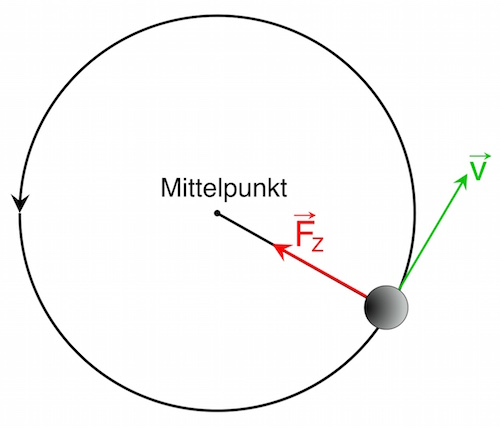
\includegraphics[width=0.3\textwidth]{Zentripetalkraft.jpg}
	  %\caption{Zentripetalkraft $F_z$}
   \end{wrapfigure}
Ohne äußere Kraft behält ein Körper seinen Bewegungszustand bei, das heißt, er bleibt in Ruhe oder in geradlinig gleichförmiger Bewegung.\\
Bei einem Körper, der sich auf einer Kreisbahn bewegt, ändert sich jedoch ständig die Richtung. Es muss also eine Kraft geben, die den Körper auf diese Kreisbahn zwingt.\\
Lässt man beispielsweise einen Körper an einem Faden um einen Mittelpunkt herum kreisen, muss man diesen aktiv zum Mittelpunkt ziehen.\\
Reißt der Faden, so kann keine Kraft mehr auf den Körper wirken – der Körper bewegt sich dann in die derzeitige Richtung weiter, und zwar geradlinig und tangential zur Kreisbahn.\\
}
Die Kraft, die einen Körper auf einer Kreisbahn hält, ist stets zum Kreismittelpunkt gerichtet und heißt Zentripetalkraft $F_p$. Sie wird in diesem Beispiel vom Kraftmesser gemessen.  
   \begin{figure} 
	  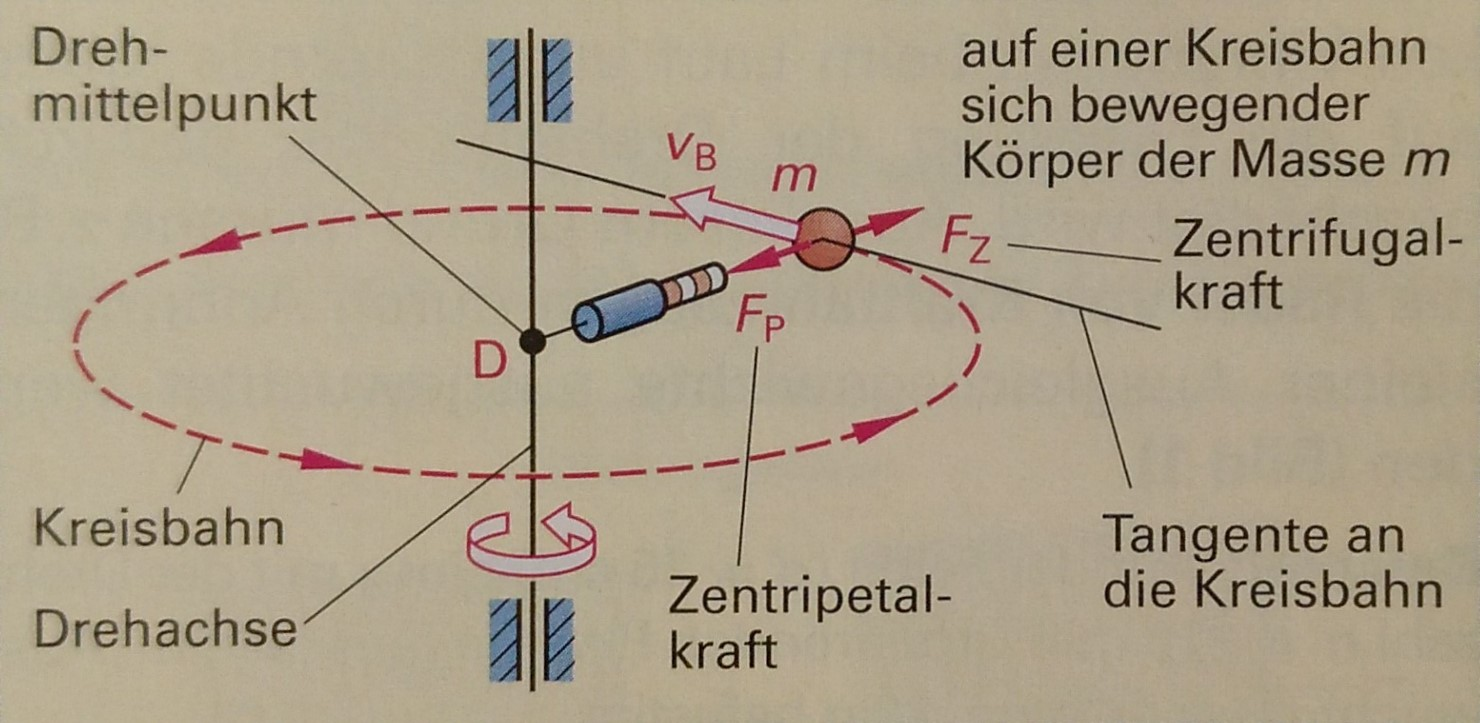
\includegraphics[width=0.5\textwidth]{Zentripetalkraft_2.jpg}
	  \caption{Kräftegleichgewicht $F_p=F_z$}
   \end{figure}
   \begin{block}{Die Zentripetalkraft}
   Die Kraft, die einen Körper auf eine Kreisbahn zwingt, heißt \textbf{Zentripetalkraft $F_p$}. Sie ist stets zum Kreismittelpunkt gerichtet und wirkt immer \textit{senkrecht} auf den momentanen \textit{Geschwindigkeitsvektor}.
   \end{block}
Bei der Frage nach den Kräften bei Kreisbewegungen denken die meisten an die \textit{Zentrifugalkraft $F_z$}. Schließlich hat diese jeder schon gespürt:\\
Bewegt man sich selbst auf einer Kreisbahn (z.B. in einem Karussell oder in einer engen Kurve), so hat man das Gefühl, dass man dabei nach \textit{außen} gezogen wird. Die Kraft, die einen nach außen zieht, ist die sog. \textbf{Zentrifugalkraft $F_z$} (\textit{Fliehkraft}).\\
Gleichzeitig spürt man jedoch auch die \textit{Zentripetalkraft $F_p$}, die einen nach innen zieht (z.B. durch den Sitz, den Gurt etc.) und auf der Kreisbahn hält. Es herrscht scheinbar ein \textit{Kräftegleichgewicht} (actio = rectio) zwischen Zentrifugal- und Zentripetalkraft, wodurch es möglich scheint, in Ruhe sitzen zu bleiben.\\
Für einen außenstehenden ruhenden Beobachter gibt es jedoch keinen Grund, eine nach außen gerichtete Kraft anzunehmen. Er erkennt kein Kräftegleichgewicht, denn für ihn ist die rotierende Person nicht in Ruhe, sondern sie ändert ständig ihre Richtung und wird demnach ständig beschleunigt.\\
Die Zentrifugalkraft wird also nur von demjenigen wahrgenommen, der sich selbst auf einer Kreisbewegung bewegt.\\
Ein Beobachter von außen benötigt zur Erkärung der Kreisbewegung lediglich die Zentripetalkraft.
   \begin{block}{Die Zentrifugalkraft (Fliehkraft)}
   Die \textbf{Zentrifugalkraft $F_z$ (Fliehkraft)} ist die Kraft, die ein sich auf einer Kreisbahn bewegender Beobachter verspürt. Sie ist der Zentripetalkraft entgegen gerichtet und gleich groß.\\
   Die Zentrifugalkraft ist eine \textbf{Trägheitskraft} und nur im rotierenden Bezugssystem erkennbar. Daher bezeichnet man sie auch als \textbf{Scheinkraft}.
   \end{block}
}

\frame{
\frametitle{Theoretische Grundlagen Zentrifugal- und Zentripetalbeschleunigung}
\begin{columns}
\column{0.5\textwidth}
\begin{figure}[htb]
\resizebox{0.9\textwidth}{!}{%
\begin{tikzpicture} 
\usetikzlibrary{calc};
\begin{scope}[scale=0.6]
\draw (0,0) circle[radius=3];
\draw (-3,0) -- (3,0);
\draw (0,-3) -- (0,3);
\coordinate (a) at (55:3);
\draw (0,0) |- (a);
\draw (0,0) -- (a);
\draw (0,-3) -- (a);
\draw (0,3) -- (a);
\draw (0,3) -| (a);
\draw[->, >=latex, thick, red] (0,3) -- node[near end, above] {$v_u$} (4,3);
\draw[->, >=latex, thick, red] (0,3) -- node[near end, left] {$a_z$} (0,0.5);
\draw (-3,0) -- (-3,-1.2);
\draw[<->, >=latex] (0,-1) -- node[above] {$r$} (-3,-1);
\path let \p1=(a) in coordinate (b) at (-3,\y1);
\draw (a) -- (b);
\draw (0,3) -- (-3,3);
\draw[<->, >=latex] ($(b) + (0.2,0)$) -- node[right] {$s$} (-2.8,3);
\draw[<-, >=latex, red] (3.2,0) arc (0:50:3.2) node[right,near start] {$\omega$};
\draw[<->, >=latex] (0,1.7) arc (90:55:1.7) node[above,midway] {$\varphi$};
\fill (a) circle[radius=0.08];
\node[below] at (a) {$C$};
\fill (0,0) circle[radius=0.08];
\node[below right] at (0,0) {$M$};
\fill (0,-3) circle[radius=0.08];
\node[below] at (0,-3) {$E$};
\fill (0,3) circle[radius=0.12];
\node[above] at (0,3) {$A$};
\path let \p1=(a) in coordinate (c) at (0,\y1);
\fill (c) circle[radius=0.08];
\node[below left] at (c) {$D$};
\path let \p1=(a) in coordinate (d) at (\x1,3);
\node[above] at (d) {$B$};
\fill (d) circle[radius=0.08];
\end{scope}
\end{tikzpicture}
}%
\caption{Zentripetalbeschleunigung $a_z$}
\end{figure}
\column{0.5\textwidth}
\begin{align*}
s&=\dfrac{a_z}{2}\cdot t^{2}\\
\overline{DC}^{2}&=\overline{AD}\cdot\overline{DE}\\
\overline{AD}&=s=\dfrac{a_z}{2}\cdot t^{2}\\
\overline{AB}^{2}&=\dfrac{a_z}{2}\cdot t^{2}\cdot \overline{DE}\\
\overline{AB}&=v_u\cdot t ,\quad \overline{DE}=2\cdot r-s\\
(v_u\cdot t)^{2}&=\dfrac{a_z}{2}\cdot t^{2}\cdot(2\cdot r-s)\\
\Aboxed{a_z&=\frac{v_u^2}{r},\quad a_z=r\cdot\omega^2}
\end{align*}
\end{columns}
}

\frame
{
  \frametitle{Theoretische Grundlagen Zentrifugal- und Zentripetalbeschleunigung}
Die auf den Körper während der Drehbewegung wirkende Zentrifugalkraft (Trägheitskraft) ist gegeben durch:
\begin{align}
F_z=m\cdot a_z=m\cdot\dfrac{v^{2}}{r}=m\cdot r\cdot \omega^{2}
\end{align}
Nach Division durch die Masse $m$ erhalten wir den Ausdruck für die radial nach außen gerichtete Beschleunigung $a_z$. Der Betrag der Zentrifugalbeschleunigung $a_z$ ist gleich dem Betrag der Zentripetalbeschleunigung $a_p$:
\begin{align}
a_z=\vert a_p\vert=r\cdot \omega^{2}
\end{align}
Daran erkennt man, dass die radial nach außen gerichtete Beschleunigung $a_z$ linear mit dem Radius $r$ und quadratisch mit der Winkelgeschwindigkeit (Drehrate) $\omega$ zunimmt.
}

\frame
{
\frametitle{Messungen mit dem Smartphone}

Ein Smartphone besitzt einen dreiachsigen Beschleunigungssensor zur Bestimmung der linearen Beschleunigung $\overrightarrow{a}=(a_{x},a_{y},a_{z})$ und einen dreiachsigen Drehratensensor (Gyro) zur Bestimmung der Drehgeschwindigkeit oder Winkelgeschwindigkeit $\overrightarrow{\omega}=(\omega_{x},\omega_{y},\omega_{z})$ entlang jeder Koordinatenachse. Die Orientierung dieser Sensoren ist in (1) und (2) gezeigt:

\begin{tabular}{@{} *{2}{C{.5\linewidth}} }
  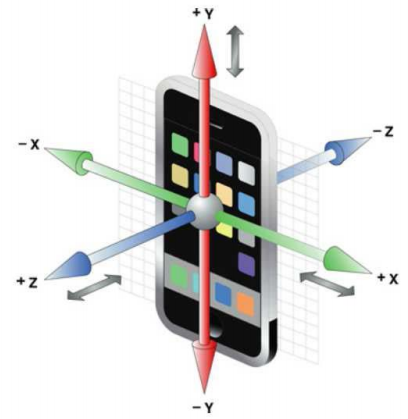
\includegraphics[width=.45\linewidth]{Smartphone_1.png} &
    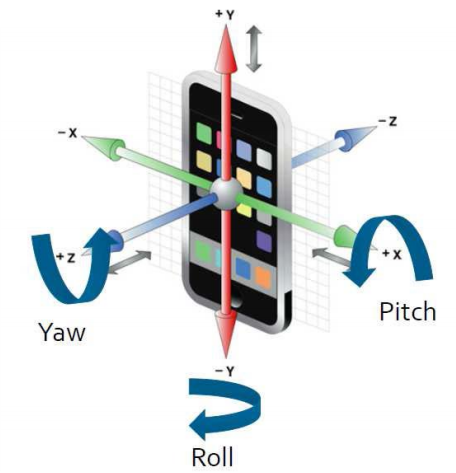
\includegraphics[width=.45\linewidth]{Smartphone_2.png} \\[\abovecaptionskip]
  Orientierung der Beschleunigungssensoren & Orientierung der Drehratensensoren
\end{tabular}
}

\frame
{
\frametitle{Messungen mit dem Smartphone}

\textbf{Versuchsaufbau}\\
Der Versuchsaufbau besteht aus einem PC-Lüfter auf dem ein Smartphone fixiert ist. Über die Spannungsversorgung von $\SI{5}{\volt}$ kann der Lüfter samt Smartphone in eine Drehbewegung versetzt werden. Aufgrund des Trägheitsmomentes der Anordnung, nimmt die Winkelgeschwindigkeit beim Anlegen der Spannung langsam zu und reduziert sich ebenso langsam nach dem Abschalten. 
   \begin{figure} 
	  \includegraphics[width=0.35\textwidth]{versuchsaufbau.jpg}
   \end{figure}
}

\frame[allowframebreaks]
{
\frametitle{Messungen mit dem Smartphone}

\textbf{Messung mit \phyphox}\\
Mit der \phyphox -App,  welche unter \url{www.phyphox.org} heruntergeladen werden kann, lassen sich alle Sensoren  eines Smartphones  auslesen. Die Daten lassen sich in Quasi-Echtzeit per WLAN an einen Rechner übertragen,  visualisieren, abspeichern und aus werten.
   \begin{figure} 
	  \includegraphics[width=0.6\textwidth]{phyphox.png}
   \end{figure}
Wir wählen den Versuch Zentripetalbeschleunigung. Die gewonnenen Daten werden lokal gespeichert und mit Hilfe von Gnuplot\footnote{(Eigenschreibweise: gnuplot) ist ein skript- bzw. kommandozeilengesteuertes Computerprogramm zur grafischen Darstellung von Messdaten und mathematischen Funktionen (Funktionenplotter).} grafisch dargestellt und ausgewertet.
   \begin{figure} 
	  \includesvg[width=0.55\textwidth]{Zentripedalbescheunigung.svg}
   \end{figure}
}

\frame
{
  \frametitle{Zusammenfassung Zentripetalkraft, Zentrifugalkraft}
  \begin{theorem}[Bei der Drehbewegung einer Masse wirken zwei radiale Kräfte, die gleich groß, aber entgegengesetzt gerichtet sind]
  $F_z=F_p=m\cdot\dfrac{v^{2}}{r}=m\cdot\omega^{2}\cdot r=m\cdot (2\pi\cdot n)^{2}\cdot r$
  \end{theorem}
  Dabei ist:
  \begin{description}
  \item $F_z=$ Zentrifugalkraft in N
  \item $F_p=$ Zentripetalkraft in N
  \item $m=$ Masse in kg
  \item $v=$ Umlaufgeschwindigkeit in $\frac{m}{s}$
  \item $r=$ Abstand vom Drehmittelpunkt in m
  \item $n=$ Drehzahl in $\frac{1}{s}$
  \end{description}
  \begin{tabular}{c|c|c|c|c|c}
  $F_z, F_p$ & $m$ & $v$ & $\omega$ & $r$ & $n$ \\ 
  \hline 
  $N$ & $kg$ & $\frac{m}{s}$ & $\frac{rad}{s}$ & $m$ & $\frac{1}{s}$ \\ 
  \end{tabular} 
}

\frame
{
\frametitle{Beispielaufgabe 1}
\uncover<1->
{
\textbf{Aufgabe:}\\
Auf der Felge ($d=\SI{35}{\centi\meter}$) eines mit der Drehzahl $n=\SI{2100}{\minute^{-1}}$ rotierenden Pkw-Reifens ist ein 'Auswuchtgewicht' von $\SI{20}{\gram}$ befestigt.\\
Wie groß ist die von ihm ausgehende Zentrifugalkraft?\\
}
\uncover<2->
{
\textbf{Lösung:}\\
\begin{align*}
n&=\SI{2100}{\minute^{-1}}=\dfrac{2100}{\SI{60}{s}}=\SI{35}{\second^{-1}};\quad m=\SI{20}{\gram}=\SI{0.020}{\kilo\gram}\\
r&=\dfrac{\SI{35}{\centi\meter}}{2}=\SI{17.5}{\centi\meter}=\SI{0.175}{\meter}\\
F_z&=m\cdot (2\pi\cdot n)^{2}\cdot r\\
&=\SI{0.020}{\kilo\gram}\cdot (2\pi\cdot 35)^{2}s^{-2}\cdot \SI{0.175}{\meter}\approx\SI{169}{\newton}\\
\end{align*}
}
}

\frame[allowframebreaks]
{
\frametitle{Beispielaufgabe 2}
\uncover<1->
{
\textbf{Aufgabe:}\\
Jeder kennt sicherlich das Phänomen, dass man einen mit Wasser gefüllten Eimer vertikal kreisen lassen kann, ohne dass das Wasser aus dem Eimer fließt. Der Radius ergibt sich aus der Länge des Armes und dem Henkel des Eimers und soll $\SI{1}{\meter}$ betragen.\\
Wie schnell muss der Eimer rotieren, damit kein Wasser heraus fließt?\\
}
\uncover<2->
{
\textbf{Lösung:}\\
\begin{align*}
F_z\geq F_G \Rightarrow m\cdot\dfrac{v^{2}}{r}&\geq m\cdot g\\
v&\geq\sqrt{r\cdot g}\\
v&\geq\SI{3.13}{\frac{\meter}{\second}};\quad v\geq\SI{11.3}{\frac{\kilo\meter}{\hour}}\\
\omega&=\dfrac{v}{r};\quad\omega=2\pi\cdot f\\
f&=\dfrac{v}{2\pi\cdot r}=\dfrac{\SI{3.13}{\frac{m}{s}}}{2\pi\cdot\SI{1}{\meter}}=\SI{0.5}{\hertz}\\
T&=\SI{2}{\second}
\end{align*}
}
}

\frame[allowframebreaks]
{
\frametitle{Beispielaufgabe 3}
\textbf{Aufgabe:}\\
Ein Triebwagen durchfährt eine Kurve mit dem Krümmungsradius $\SI{250}{\meter}$ Das Gleis ist genau horizontal verlegt, d.h., dass sich die beiden Schienen genau auf der gleichen Höhe befinden. Bei welcher Geschwindigkeit beginnt der Wagen zu kippen, wenn sein Schwerpunkt $\SI{1.3}{\meter}$ über der Oberkante der Schienen liegt und wenn Normalspurweite $=\SI{1435}{\milli\meter}$ (Schienenabstand) vorliegt?
\newpage
\textbf{Lösung:}\\
\begin{align*}
F_z\geq tan \alpha\cdot F_G \Rightarrow  tan \alpha=\frac{\SI{1435}{\milli\meter}}{2\cdot \SI{1.3}{\meter}}\\
F_z=m\cdot\dfrac{v^{2}}{r}\geq F_G=\frac{\SI{1435}{\milli\meter}}{2\cdot \SI{1.3}{\meter}}\cdot m\cdot g\\
v\geq\sqrt{\frac{r\cdot g\cdot 1.435}{2\cdot 1.3}}=\sqrt{\frac{\SI{250}{\meter}\cdot \SI{9.81}{\frac{\meter}{\square\second}}\cdot 1.435}{2\cdot 1.3}}\\
v\geq\SI{36.78}{\frac{\meter}{\second}}=\SI{132.43}{\frac{\kilo\meter}{\hour}}
\end{align*}

}
\end{document}
